\section{Event Observable Distributions}


\subsection{Jet Kinematics}
\begin{figure}[htbp]
  \begin{center}
    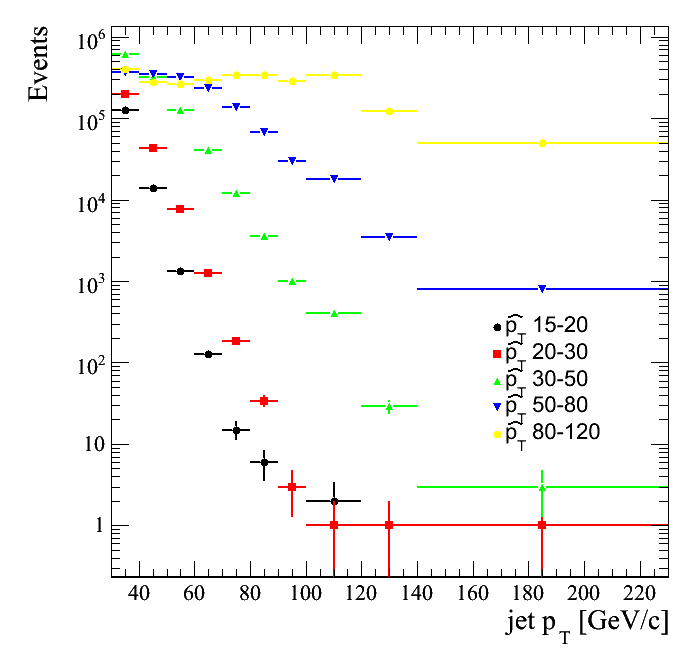
\includegraphics[width=60mm]{Figures/jet_ptqcdbinned.png}
    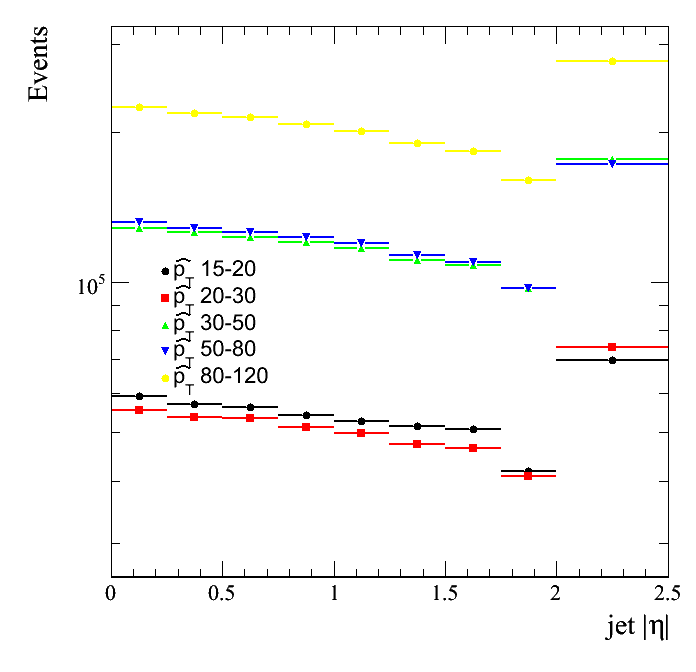
\includegraphics[width=60mm]{Figures/jet_eta_qcdbinned.png}
  \end{center}
  \caption{Jet pT from QCD.}
  \label{fig:jet_pt_QCD}
\end{figure}

\begin{figure}[htbp]
  \begin{center}
    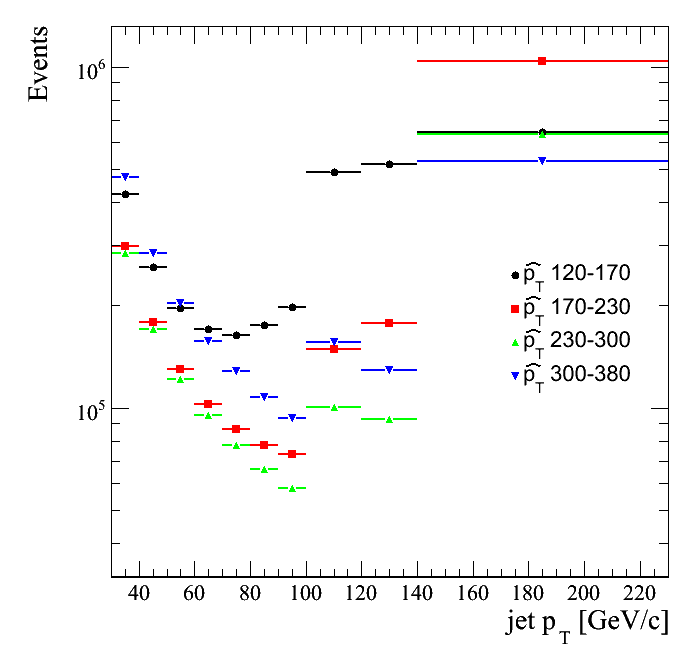
\includegraphics[width=60mm]{Figures/jet_pt2qcdbinned.png}
    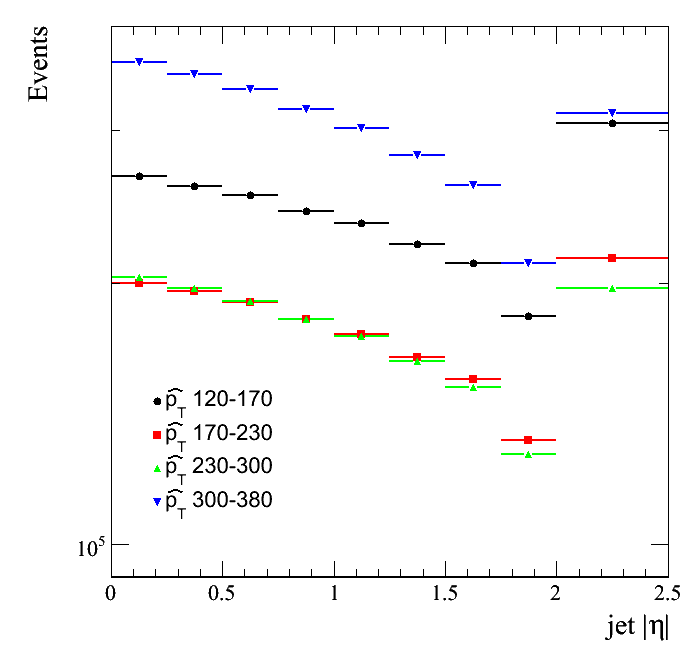
\includegraphics[width=60mm]{Figures/jet_eta_qcdbinned2.png}
  \end{center}
  \caption{Jet pT from QCD.}
  \label{fig:jet_pt_QCD2}
\end{figure}

\begin{figure}[htbp]
  \begin{center}
    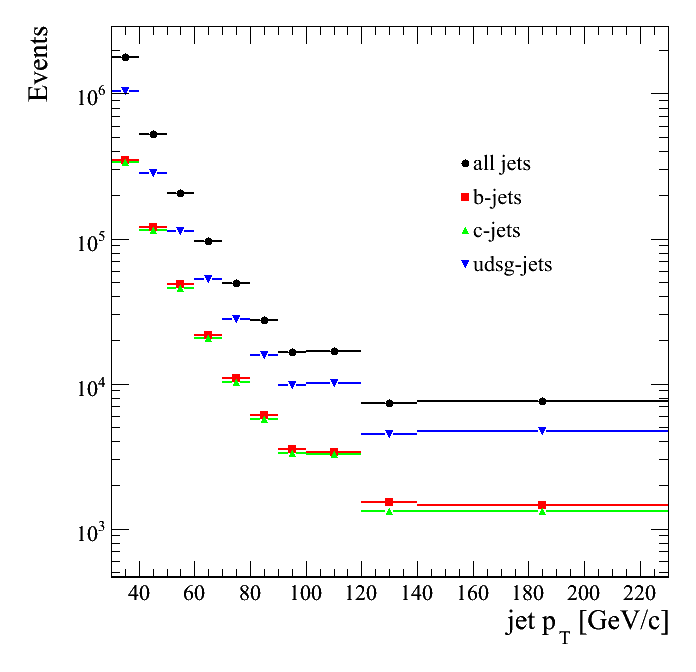
\includegraphics[width=60mm]{Figures/jet_pt_muX.png}
    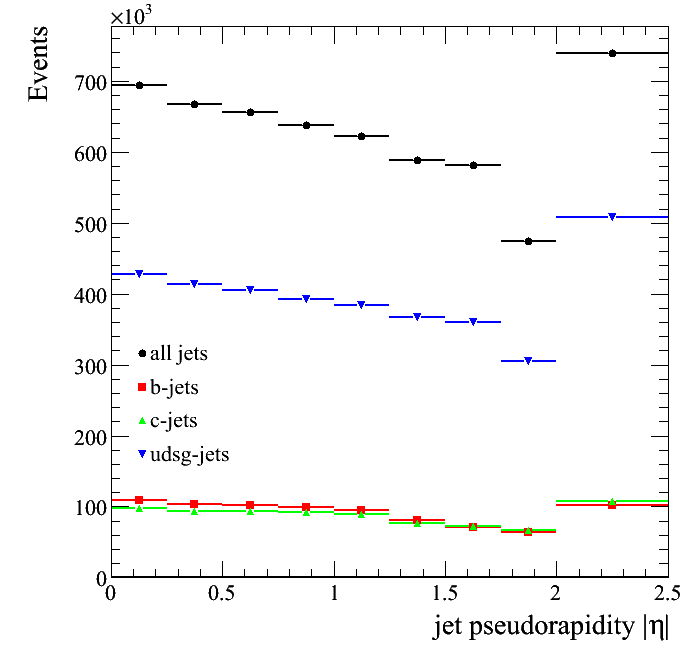
\includegraphics[width=60mm]{Figures/jet_eta_muX.png}
  \end{center}
  \caption{Jet pT and eta from muX.}
  \label{fig:jet_pt_QCD}
\end{figure}

\begin{figure}[htbp]
  \begin{center}
    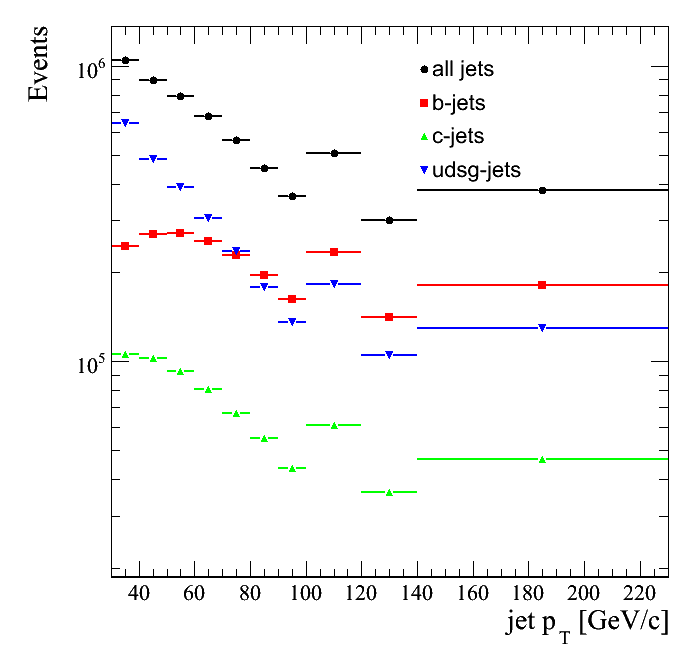
\includegraphics[width=60mm]{Figures/jet_pt_tt0j.png}
    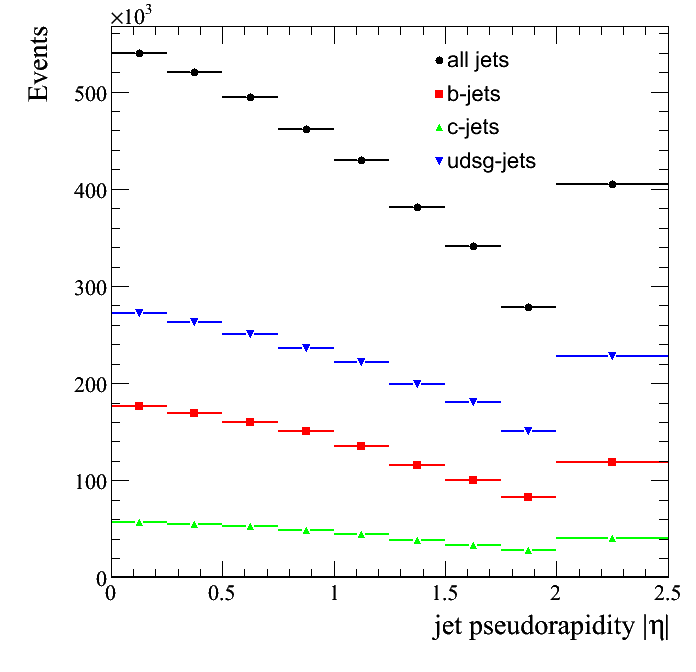
\includegraphics[width=60mm]{Figures/jet_eta_tt0j.png}
  \end{center}
  \caption{Jet pT and eta from ttbar+0jets.}
  \label{fig:jet_pt_QCD}
\end{figure}

\clearpage

\subsection{Muon $p_T$ with respect to muon+jet axis ($p_{Trel}$)}

\begin{figure}[htbp]
  \begin{center}
    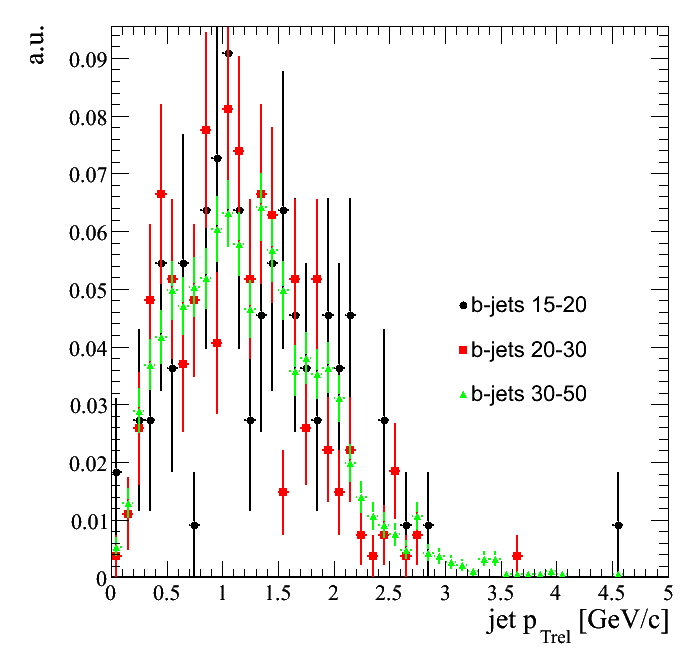
\includegraphics[width=60mm]{Figures/jet_ptrel_qcdbinned.png}
    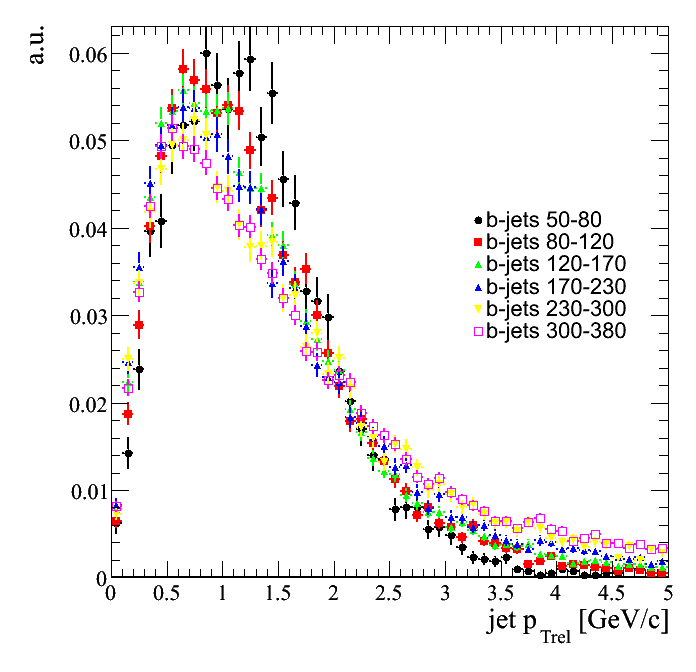
\includegraphics[width=60mm]{Figures/jet_ptrel2qcdbinned.png}
  \end{center}
  \caption{pTrel from b-jets.}
  \label{fig:jet_ptrel}
\end{figure}

\begin{figure}[htbp]
  \begin{center}
    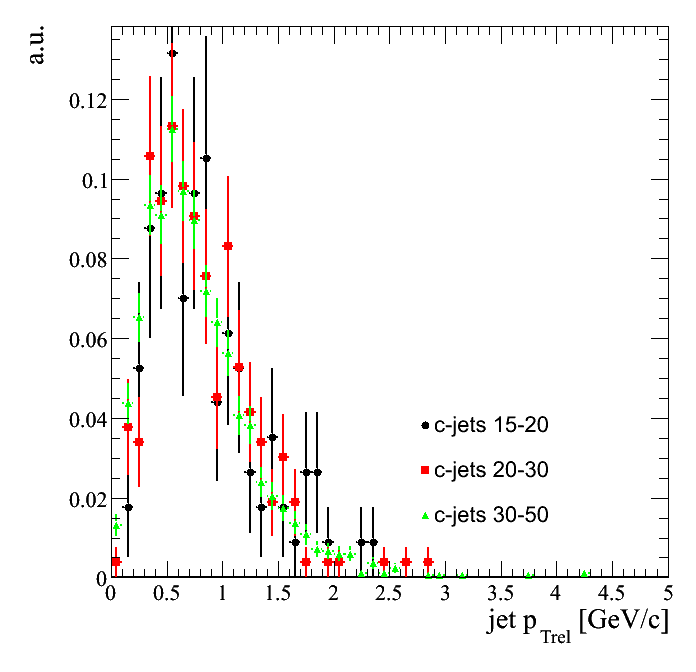
\includegraphics[width=60mm]{Figures/jet_ptrelcqcdbinned.png}
    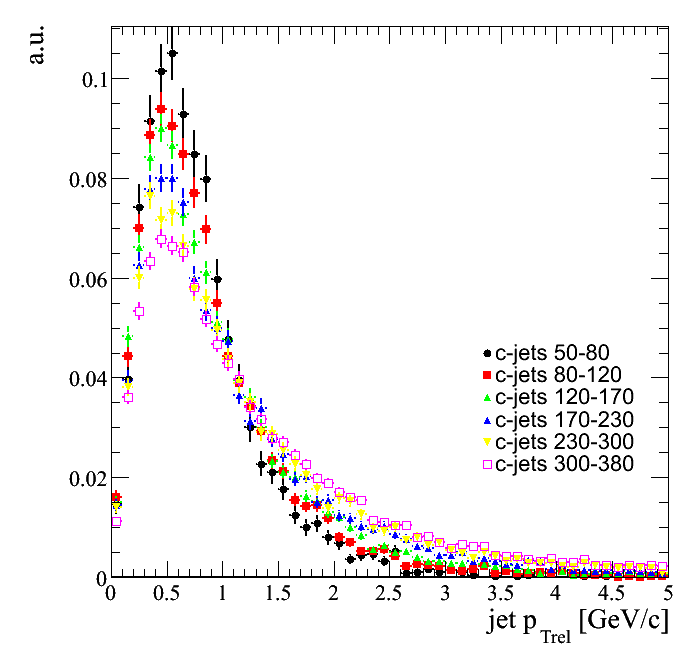
\includegraphics[width=60mm]{Figures/jet_ptrelcqcdbinned2.png}
  \end{center}
  \caption{pTrel from c-jets.}
  \label{fig:jet_ptrel}
\end{figure}


\begin{figure}[htbp]
  \begin{center}
    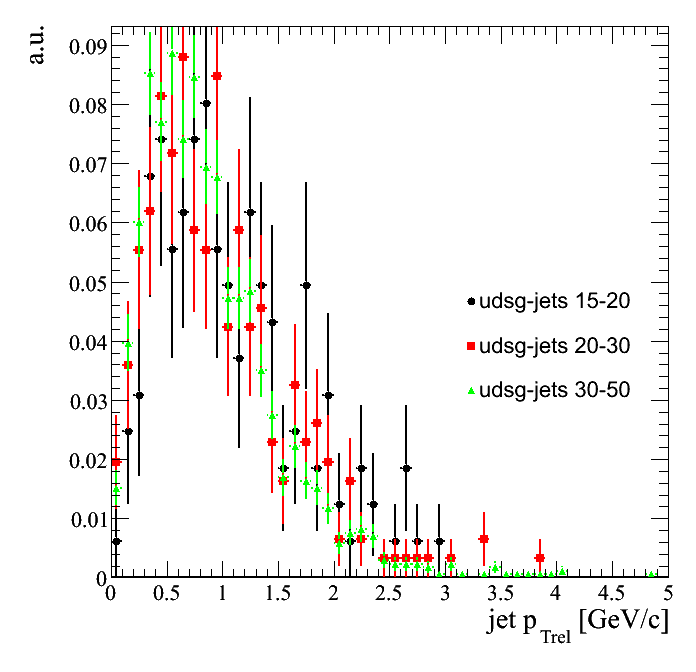
\includegraphics[width=60mm]{Figures/jet_ptreludsgqcdbinned.png}
    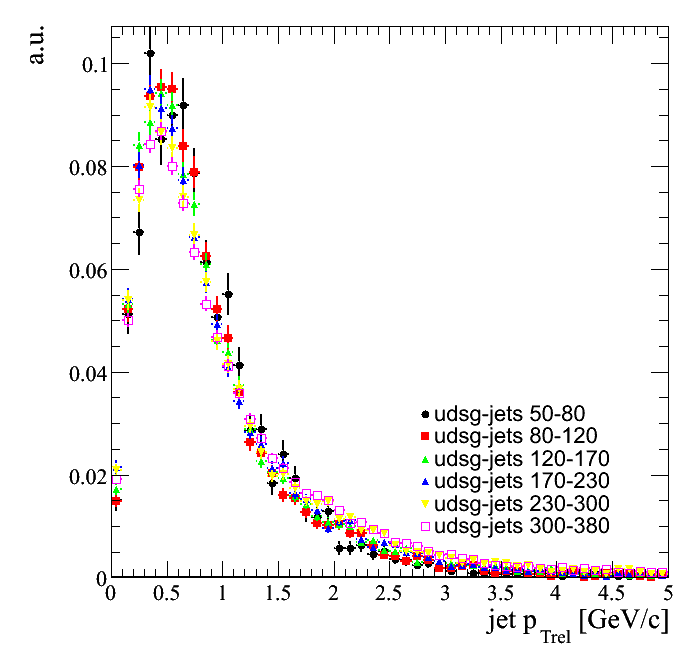
\includegraphics[width=60mm]{Figures/jet_ptreludsgqcdbinned2.png}
  \end{center}
  \caption{pTrel from udsg-jets.}
  \label{fig:jet_ptrel}
\end{figure}

\begin{figure}[htbp]
  \begin{center}
    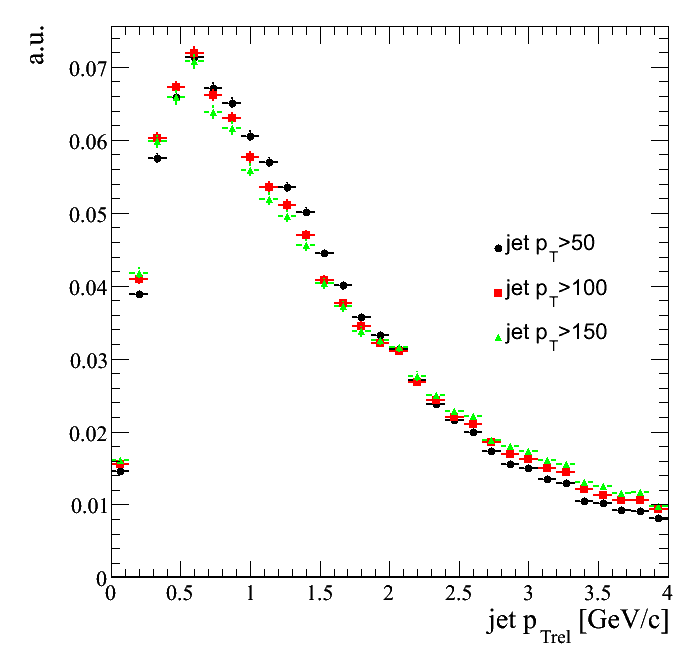
\includegraphics[width=60mm]{Figures/jet_ptrelb_jetcuts.png}
    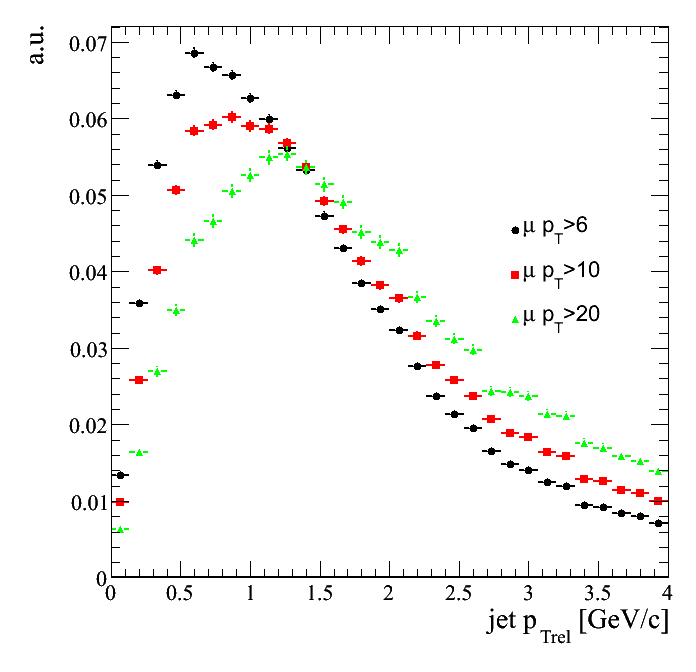
\includegraphics[width=60mm]{Figures/jet_ptrelb_mucuts.png}
  \end{center}
  \caption{pTrel from b-jets for jet and muon cuts.}
  \label{fig:jet_ptrel}
\end{figure}

\begin{figure}[htbp]
  \begin{center}
    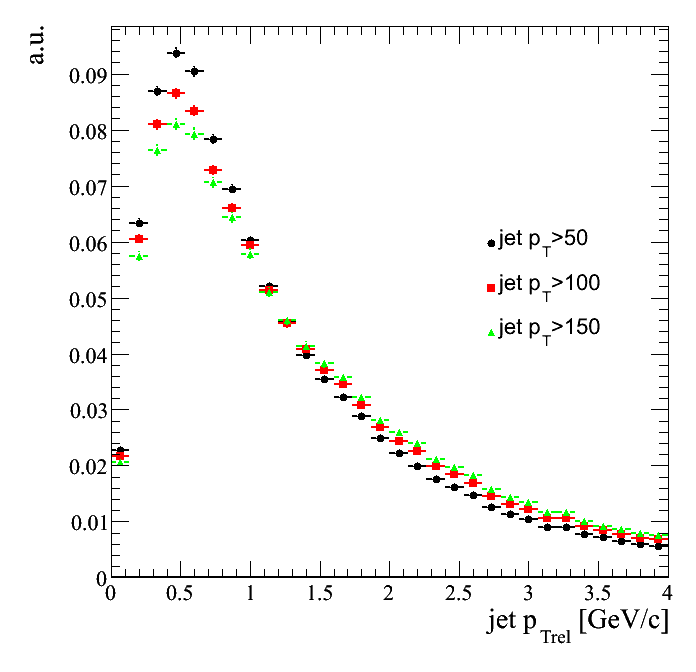
\includegraphics[width=60mm]{Figures/jet_ptrelc_jetcuts.png}
    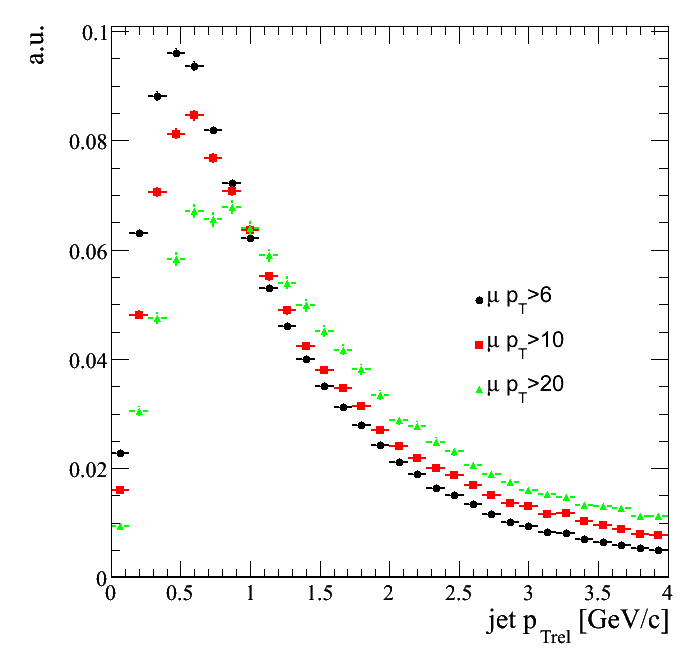
\includegraphics[width=60mm]{Figures/jet_ptrelc_mucuts.png}
  \end{center}
  \caption{pTrel from c-jets for jet and muon cuts.}
  \label{fig:jet_ptrel}
\end{figure}

\begin{figure}[htbp]
  \begin{center}
    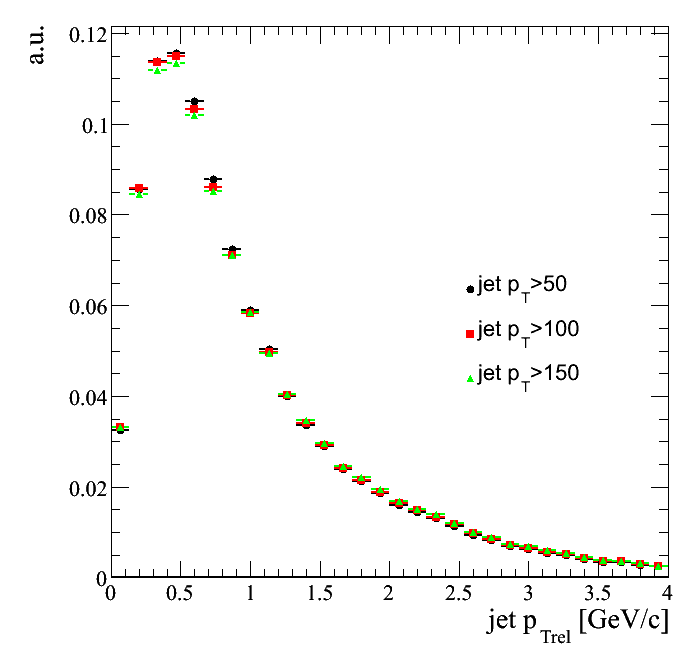
\includegraphics[width=60mm]{Figures/jet_ptreludsg_jetcuts.png}
    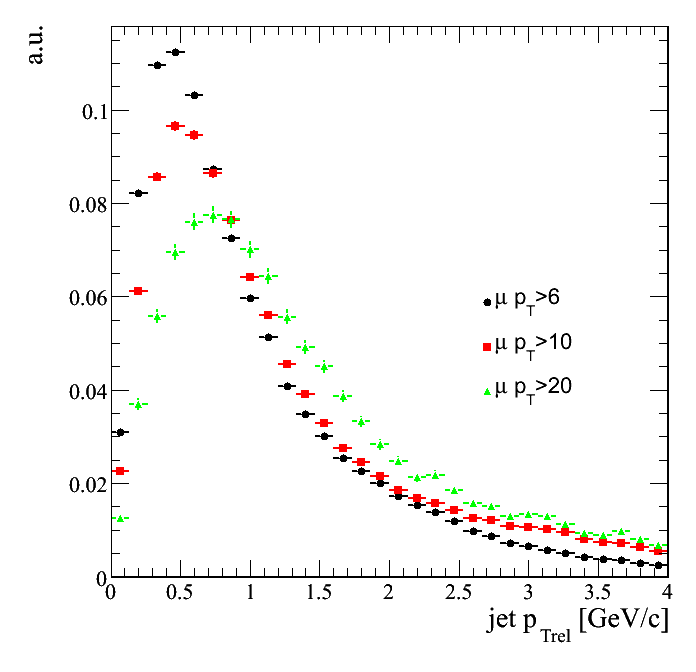
\includegraphics[width=60mm]{Figures/jet_ptreludsg_mucuts.png}
  \end{center}
  \caption{pTrel from udsg-jets for jet and muon cuts.}
  \label{fig:jet_ptrel}
\end{figure}

\begin{figure}[htbp]
  \begin{center}
    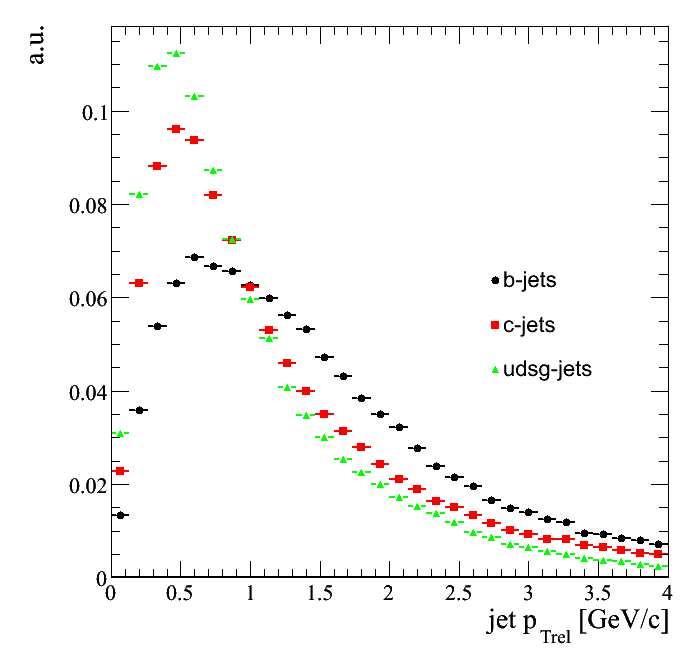
\includegraphics[width=60mm]{Figures/jet_ptrel_mu6.png}
    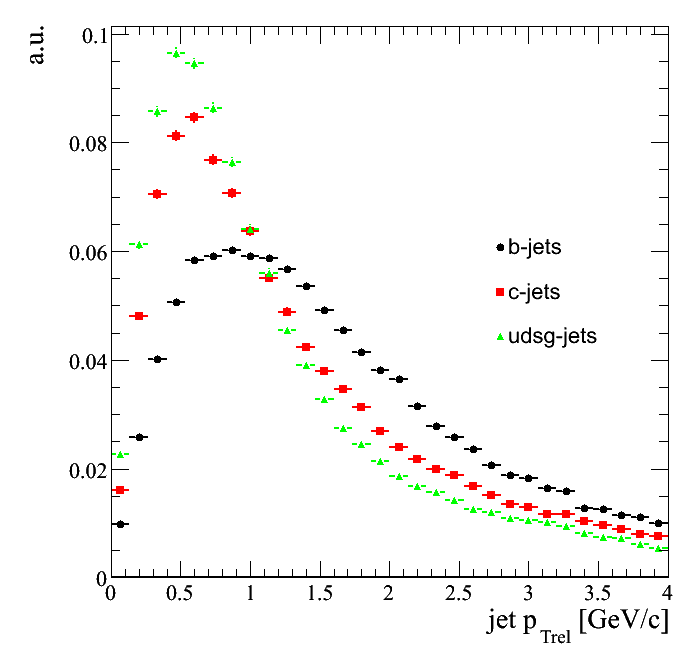
\includegraphics[width=60mm]{Figures/jet_ptrel_mu10.png}
    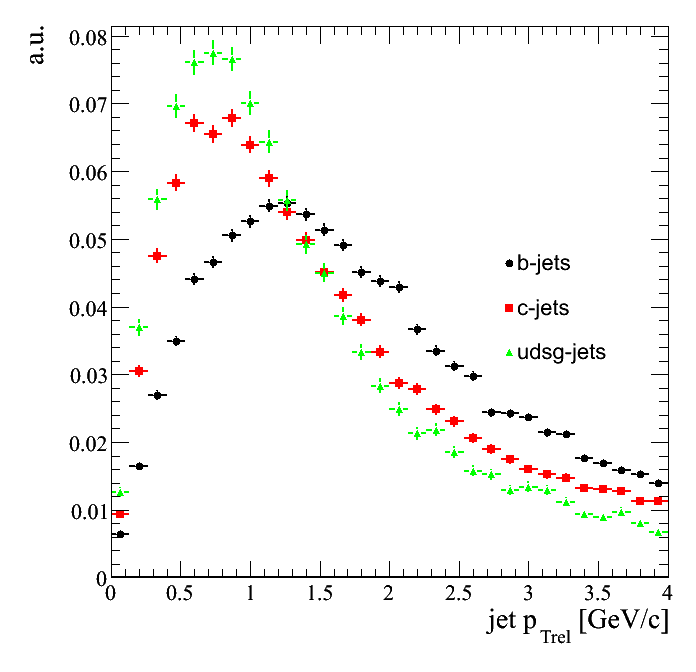
\includegraphics[width=60mm]{Figures/jet_ptrel_mu20.png}
  \end{center}
  \caption{pTrel for muon cuts.}
  \label{fig:jet_ptrel}
\end{figure}

\begin{figure}[htbp]
  \begin{center}
    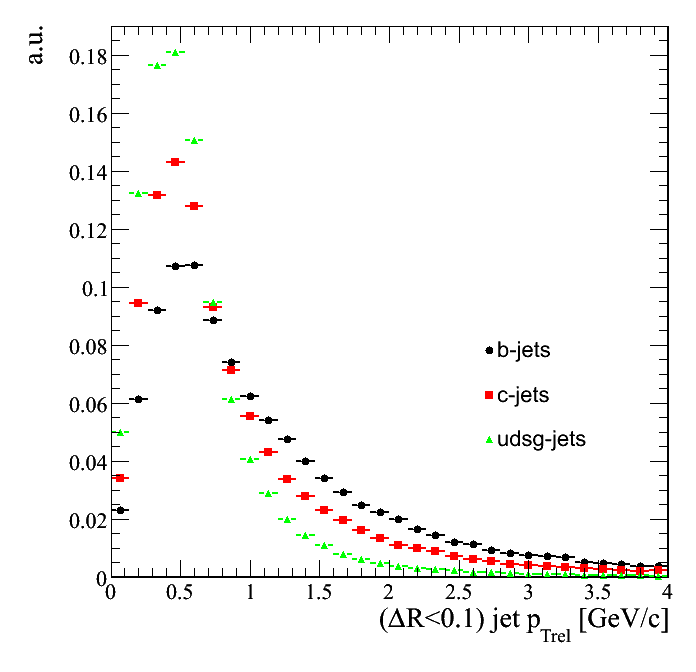
\includegraphics[width=60mm]{Figures/jet_ptrel_deltaR1.png}
    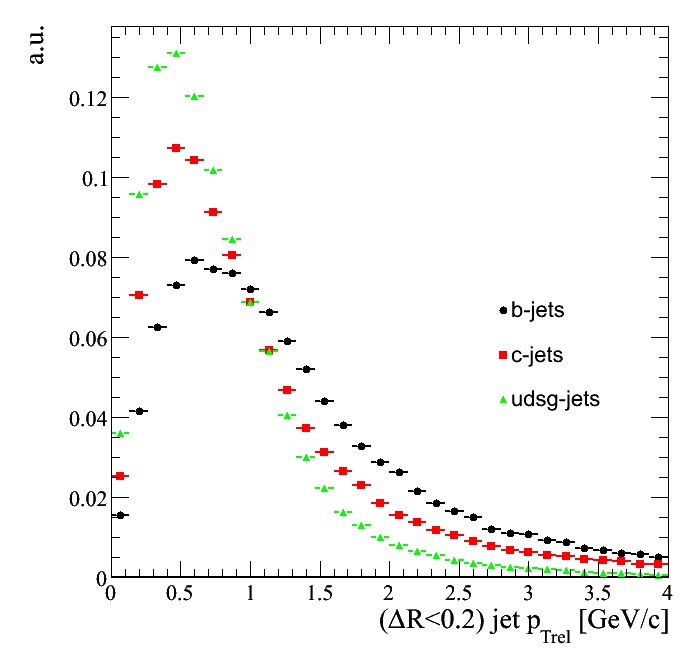
\includegraphics[width=60mm]{Figures/jet_ptrel_deltaR2.png}
    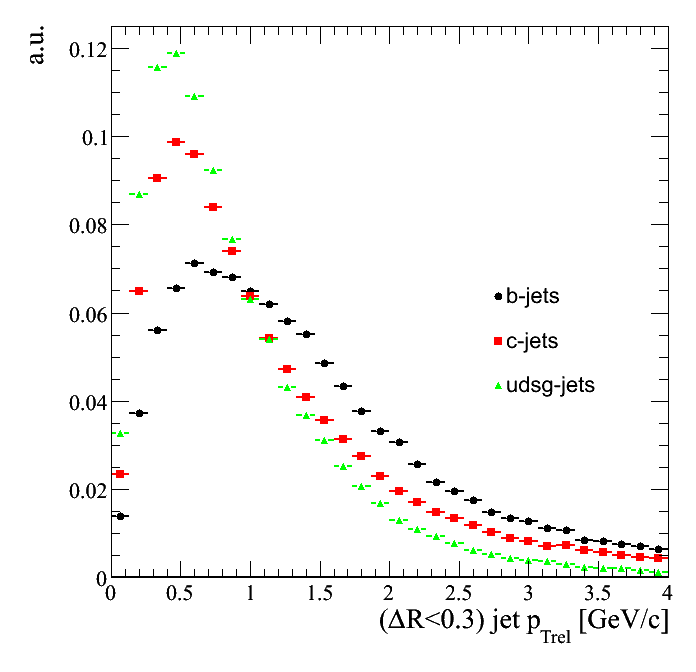
\includegraphics[width=60mm]{Figures/jet_ptrel_deltaR3.png}
  \end{center}
  \caption{pTrel for deltaR cuts.}
  \label{fig:jet_ptrel}
\end{figure}

\begin{figure}[htbp]
  \begin{center}
    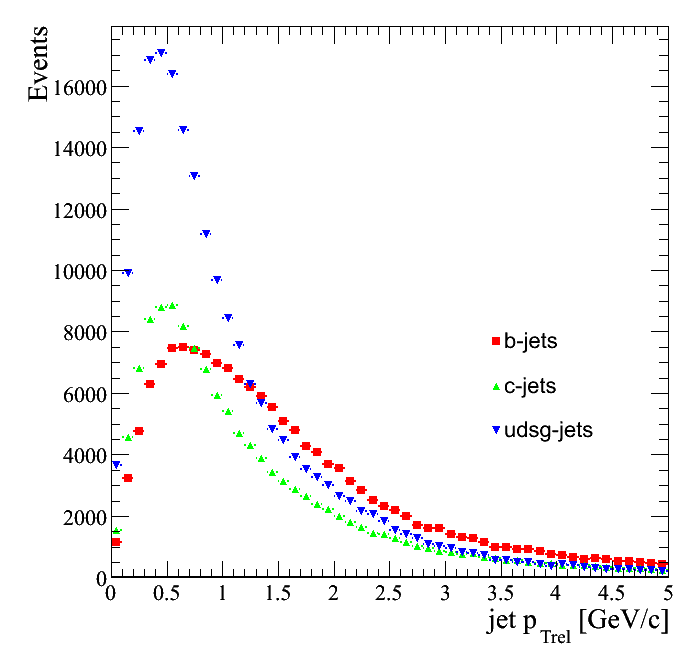
\includegraphics[width=60mm]{Figures/jet_ptrel_allqcd.png}
    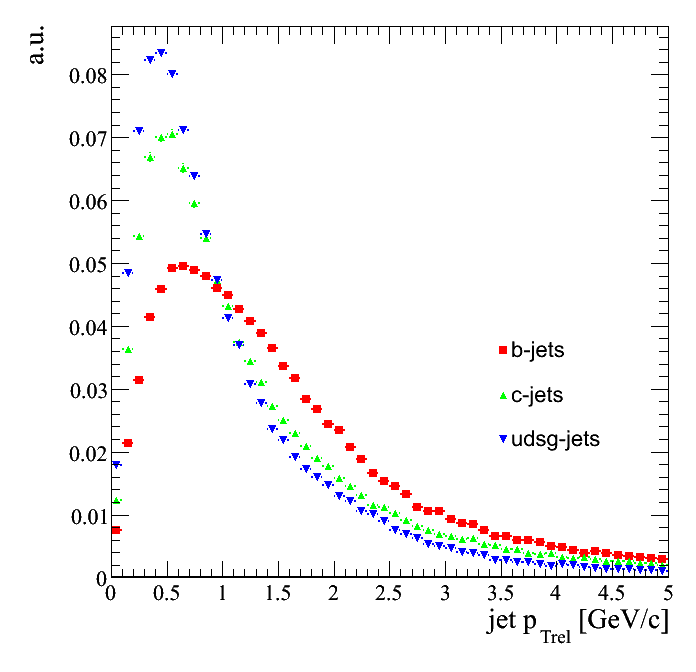
\includegraphics[width=60mm]{Figures/jet_ptrel_norm_allqcd.png}
  \end{center}
  \caption{pTrel from all QCD.}
  \label{fig:jet_ptrel}
\end{figure}


\begin{figure}[htbp]
  \begin{center}
    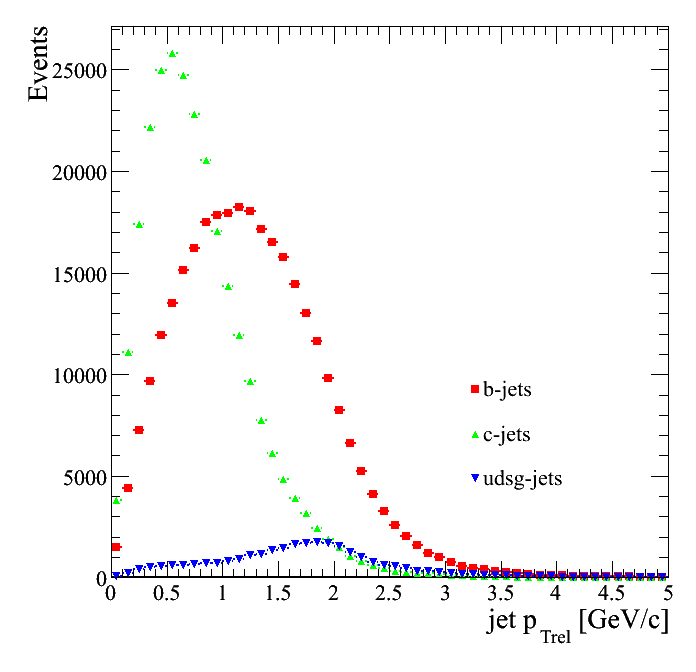
\includegraphics[width=60mm]{Figures/jet_ptrel_muX.png}
    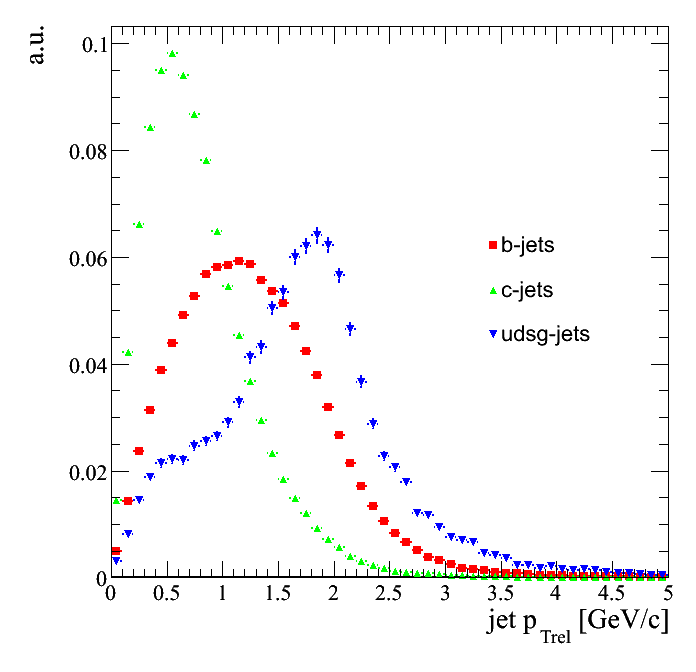
\includegraphics[width=60mm]{Figures/jet_ptrel_norm_muX.png}
  \end{center}
  \caption{pTrel from muX.}
  \label{fig:jet_ptrel}
\end{figure}


\begin{figure}[htbp]
  \begin{center}
    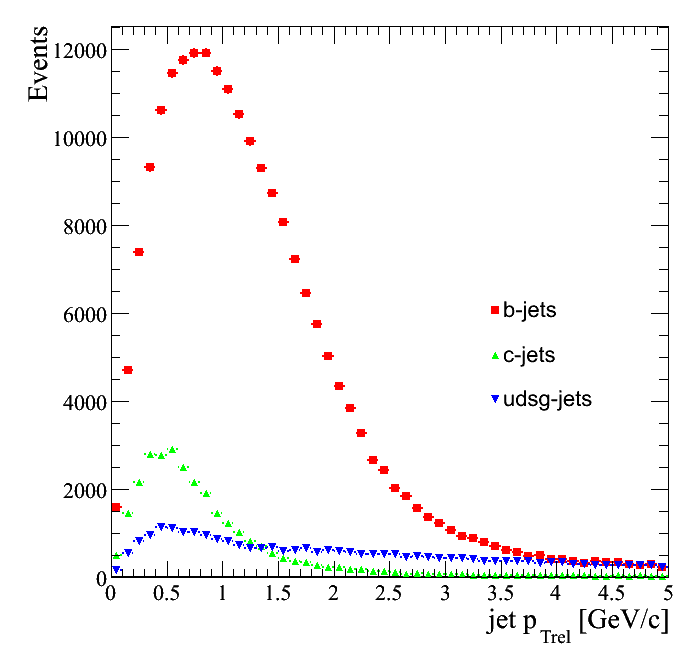
\includegraphics[width=60mm]{Figures/jet_ptrel_tt0j.png}
    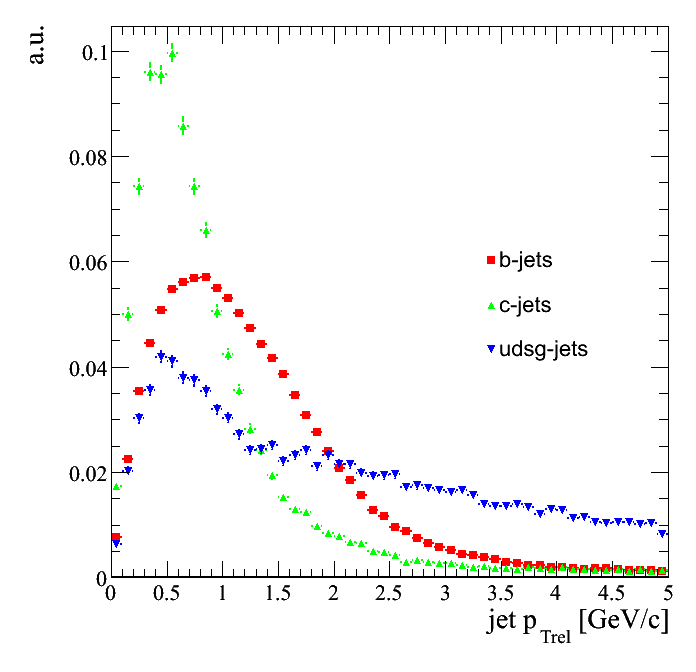
\includegraphics[width=60mm]{Figures/jet_ptrel_norm_tt0j.png}
  \end{center}
  \caption{pTrel from muX.}
  \label{fig:jet_ptrel}
\end{figure}


\clearpage

\section{System 8 Results}
\begin{figure}[htbp]
  \begin{center}
    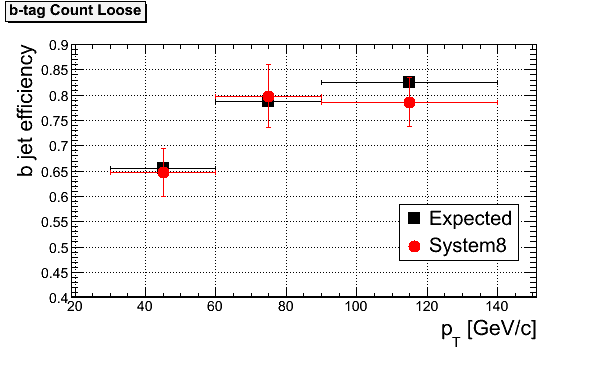
\includegraphics[width=70mm]{Figures/TCL_Tag.png}
    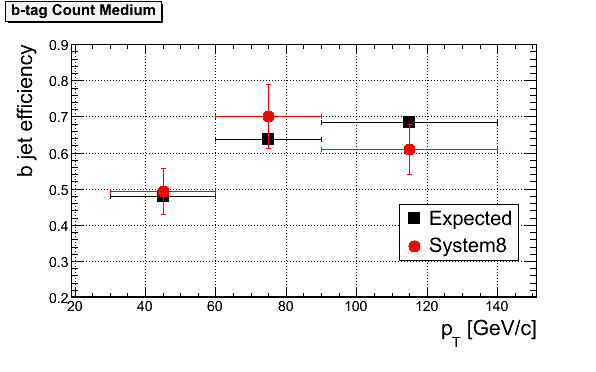
\includegraphics[width=70mm]{Figures/TCM_Tag.png}
    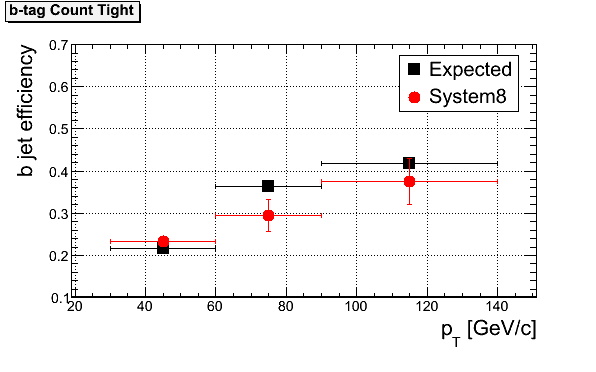
\includegraphics[width=70mm]{Figures/TCT_Tag.png}
    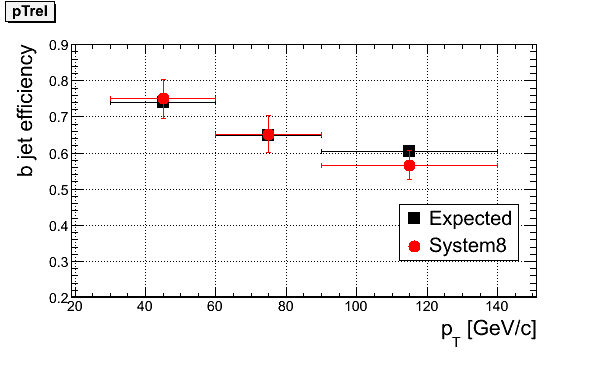
\includegraphics[width=70mm]{Figures/pTrel.png}
  \end{center}
  \caption{Measured and expected b$-$tag efficiency from System8 as a function of jet $p_T $ (requiring $p_T $ $> $ 30 GeV/c).}
  \label{fig:S8_TC_results}
\end{figure}


\begin{figure}[htbp]
  \begin{center}
    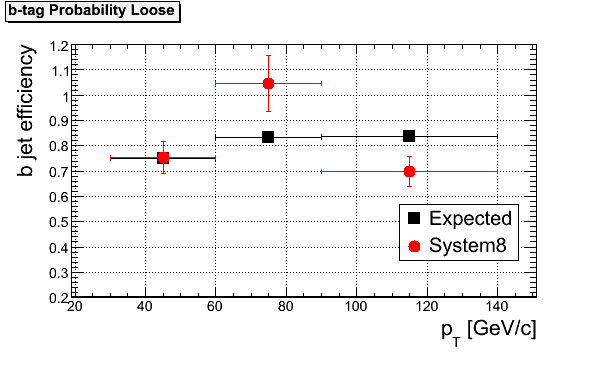
\includegraphics[width=70mm]{Figures/JPL_Tag.png}
    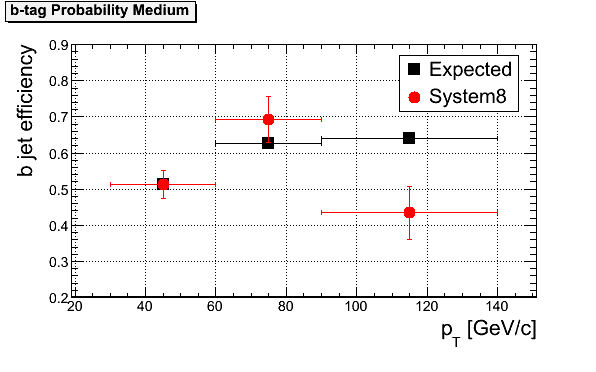
\includegraphics[width=70mm]{Figures/JPM_Tag.png}
    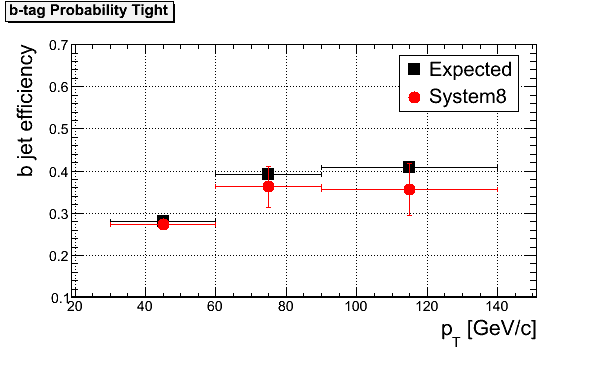
\includegraphics[width=70mm]{Figures/JPT_Tag.png}
  \end{center}
  \caption{Measured and expected b$-$tag efficiency from System8 as a function of jet $p_T $ (requiring $p_T $ $> $ 30 GeV/c).}
  \label{fig:S8_JP_results}
\end{figure}


\begin{figure}[htbp]
  \begin{center}
    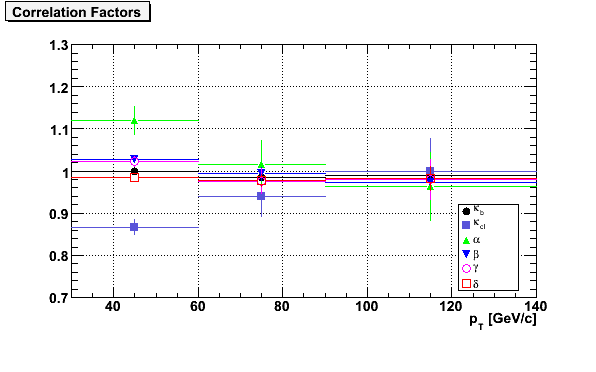
\includegraphics[width=80mm]{Figures/TCM_correlations_ppmux.png}
  \end{center}
  \caption{correlation factors.}
  \label{fig:correlation}
\end{figure}
